\documentclass[11pt,a4paper]{article}

% Paquetes básicos
\usepackage[utf8]{inputenc}
\usepackage[spanish,es-tabla]{babel}
\usepackage{amsmath, amssymb, amsfonts}
\usepackage{geometry}
\geometry{top=2.5cm, bottom=2.5cm, left=2.5cm, right=2.5cm}

% Manejo de imágenes y PDFs
\usepackage{graphicx}
\usepackage{float}
\usepackage{pdfpages}
\usepackage{adjustbox}

\begin{document}

% ---------------------------------------------------------
% CARÁTULA
% ---------------------------------------------------------
% Se incluye el PDF de la carátula compartida por el grupo

\includepdf[pages=-]{Caratula.pdf}

% ---------------------------------------------------------
% EJERCICIO 4: Naive Bayes
% ---------------------------------------------------------
\section*{4. Aplicación de un modelo Naive Bayes}

Para la resolución de este ejercicio se aplicó el modelo Naïve Bayes considerando el atributo \textit{Color} como discreto y el atributo \textit{Esfericidad} como continuo, asumiendo que este último sigue una distribución Normal. 

Los cálculos detallados de las densidades de probabilidad y los productos de verosimilitud correspondientes a cada clase fueron desarrollados de forma manuscrita. Los mismos pueden consultarse de forma detallada en el \textbf{Anexo: Procedimientos Manuscritos} al final de este documento.

\subsection*{a) Clases Equiprobables: P(Pera) = 0.5 y P(Manzana) = 0.5}

Tras aplicar el teorema de Bayes y la hipótesis MAP sobre los ejemplos dados, se obtuvieron los siguientes resultados:

\begin{table}[H]
\centering
\begin{adjustbox}{width=\textwidth}
\begin{tabular}{|l|c|c|c|c|c|c|}
\hline
\textbf{Color} & \textbf{Esfericidad} & \textbf{P(x | Pera)} & \textbf{P(x | Manzana)} & \textbf{P(x|Pera)*P(P)} & \textbf{P(x|Manz)*P(M)} & \textbf{Predicción} \\ \hline
Amarillo & 0.6 & 0.12098 & 1.00632 & 0.06049 & 0.50316 & \textbf{Manzana} \\ \hline
Mezcla & 0.8 & 1.19682 & 0.00000 & 0.59841 & 0.00000 & \textbf{Pera} \\ \hline
\end{tabular}
\end{adjustbox}
\caption{Resultados obtenidos con probabilidades a priori equiprobables.}
\end{table}

\subsection*{b) Clases NO Equiprobables: P(Manzana) = 0.01 y P(Pera) = 0.99}

En este escenario, se observa cómo la probabilidad a priori de la clase Pera tiene un peso determinante en la clasificación final, incluso cuando los atributos individuales presentan una mayor verosimilitud para la clase Manzana.

\begin{table}[H]
\centering
\begin{adjustbox}{width=\textwidth}
\begin{tabular}{|l|c|c|c|c|c|c|}
\hline
\textbf{Color} & \textbf{Esfericidad} & \textbf{P(x | Pera)} & \textbf{P(x | Manzana)} & \textbf{P(x|Pera)*P(P)} & \textbf{P(x|Manz)*P(M)} & \textbf{Predicción} \\ \hline
Amarillo & 0.6 & 0.12098 & 1.00632 & 0.11977 & 0.01006 & \textbf{Pera} \\ \hline
Mezcla & 0.8 & 1.19682 & 0.00000 & 1.18485 & 0.00000 & \textbf{Pera} \\ \hline
\end{tabular}
\end{adjustbox}
\caption{Resultados obtenidos con sesgo en las probabilidades a priori.}
\end{table}

\newpage
% ---------------------------------------------------------
% EJERCICIO 5
% ---------------------------------------------------------
\section*{5. Modelo de Naive Bayes}
% Espacio reservado para el desarrollo de los integrantes Silicaro Pera y Pacchialat.
\subsection*{a) Desarrollo del Modelo}
El modelo que buscamos desarrollar se basa en el Teorema de Bayes:

\[
P(c \mid X) = \frac{P(X \mid c)\cdot P(c)}{P(X)}
\]

Dado que $P(X)$ es constante para todas las clases, esta se cancelará en los cálculos, por lo que se utiliza la proporcionalidad:

\[
P(c \mid X) \propto P(X \mid c)\cdot P(c)
\]

Hay una consideración para tener en cuenta y es que estaremos usando el enfoque Naive Bayes. Se le llama "naive" porque estaremos tomando el Teorema de Bayes y asumiendo independencia condicional entre los atributos. Esto no es necesariamente realista (por ejemplo, podría plantearse que existe una relación entre la Luminosidad y la Temperatura de una estrella), pero asumirlo simplifica enormemente los cálculos.

\[
P(X \mid c) = \prod_{i} P(x_i \mid c)
\]

Por lo tanto:

\[
P(c \mid X) \propto P(c)\cdot P(T \mid c)\cdot P(L \mid c)\cdot P(H \mid c)
\]

\subsection*{5.1 Probabilidades a Ojo}
Estas no nacen de algún calculo complejo, son simplemente la frecuencia natural con la que se presentan los casos del set de datos.
\[
P(K) = 0.6 \quad ; \quad P(F) = 0.4
\]

\subsection*{5.2 Modelado de Variables}

\subsection*{a) Variables Continuas}

\[
P(x \mid c)=\frac{1}{\sqrt{2\pi}\sigma_c} \exp\left(-\frac{(x-\mu_c)^2}{2\sigma_c^2}\right)
\]
Estamos tratando con un atributo continuo, de modo que nuestro clasificador NB debe suponer que dicho atributo sigue una distribución normal. De esto se deriva un inconveniente: los datos no siempre siguen una distribución normal; pero bastará para establecer un modelo.

\subsection*{b) Variable Categórica}

\[
P(H=h \mid c)=\frac{n(H=h, c)}{n(c)}
\]
Esta técnica se conoce como estimación por máxima verosimilitud. Debido a que estamos trabajando con pocos registros, el estimador de Laplace resultaría más adecuado. Sin embargo, enunciado mediante, omitiremos el uso del mismo.


\subsection*{5.3 Tabla de Resultados}

\begin{table}[h]
\centering
\begin{tabular}{|l|c|c|}
\hline
\textbf{Atributo / Valor} & \textbf{Clase F} & \textbf{Clase K} \\
\hline
Temperatura $\mu$ & 5100 & 2866.67 \\
Temperatura $\sigma$ & 2086.86 & 1231.08 \\
Habitable = Si & 0.25 & 0.50 \\
Habitable = No & 0.75 & 0.50 \\
Luminosidad $\mu$ & 11.75 & 3.33 \\
Luminosidad $\sigma$ & 7.63 & 1.49 \\
\hline
\end{tabular}
\caption{Parámetros por atributo y clase}
\end{table}

\begin{table}[h]
\centering
\begin{tabular}{|l|c|}
\hline
\textbf{Clase} & \textbf{Probabilidad} \\
\hline
$P(\text{Clase F})$ & 0.40 \\
$P(\text{Clase K})$ & 0.60 \\
\hline
\end{tabular}
\caption{Probabilidades a priori de clase}
\end{table}

\newpage

\subsection*{b) Procesamiento de Ejemplos}

\begin{table}[h]
\centering
\begin{tabular}{|c|c|c|c|c|c|c|c|}
\hline
Temp & Habitable & Lum & $P(x|F)$ & $P(x|K)$ & $P(x|F)P(F)$ & $P(x|K)P(K)$ & Pred \\
\hline
1900 & No & 1 & 8.57e-7 & 9.36e-6 & 3.43e-7 & 5.62e-6 & K \\
2300 & No & 2 & 1.35e-6 & 2.61e-5 & 5.40e-7 & 1.57e-5 & K \\
5500 & No & 5 & 4.98e-6 & 2.36e-6 & 1.99e-6 & 1.40e-6 & F \\
\hline
\end{tabular}
\caption{Clasificación de los tres primeros ejemplos}
\end{table}

% ---------------------------------------------------------
% ANEXO: PROCEDIMIENTOS MANUSCRITOS
% ---------------------------------------------------------
\newpage
\section*{Anexo: Procedimientos Manuscritos}

A continuación se adjuntan las capturas de los procedimientos y cálculos analíticos realizados manualmente para la resolución del Ejercicio 4.

\begin{figure}[H]
    \centering
    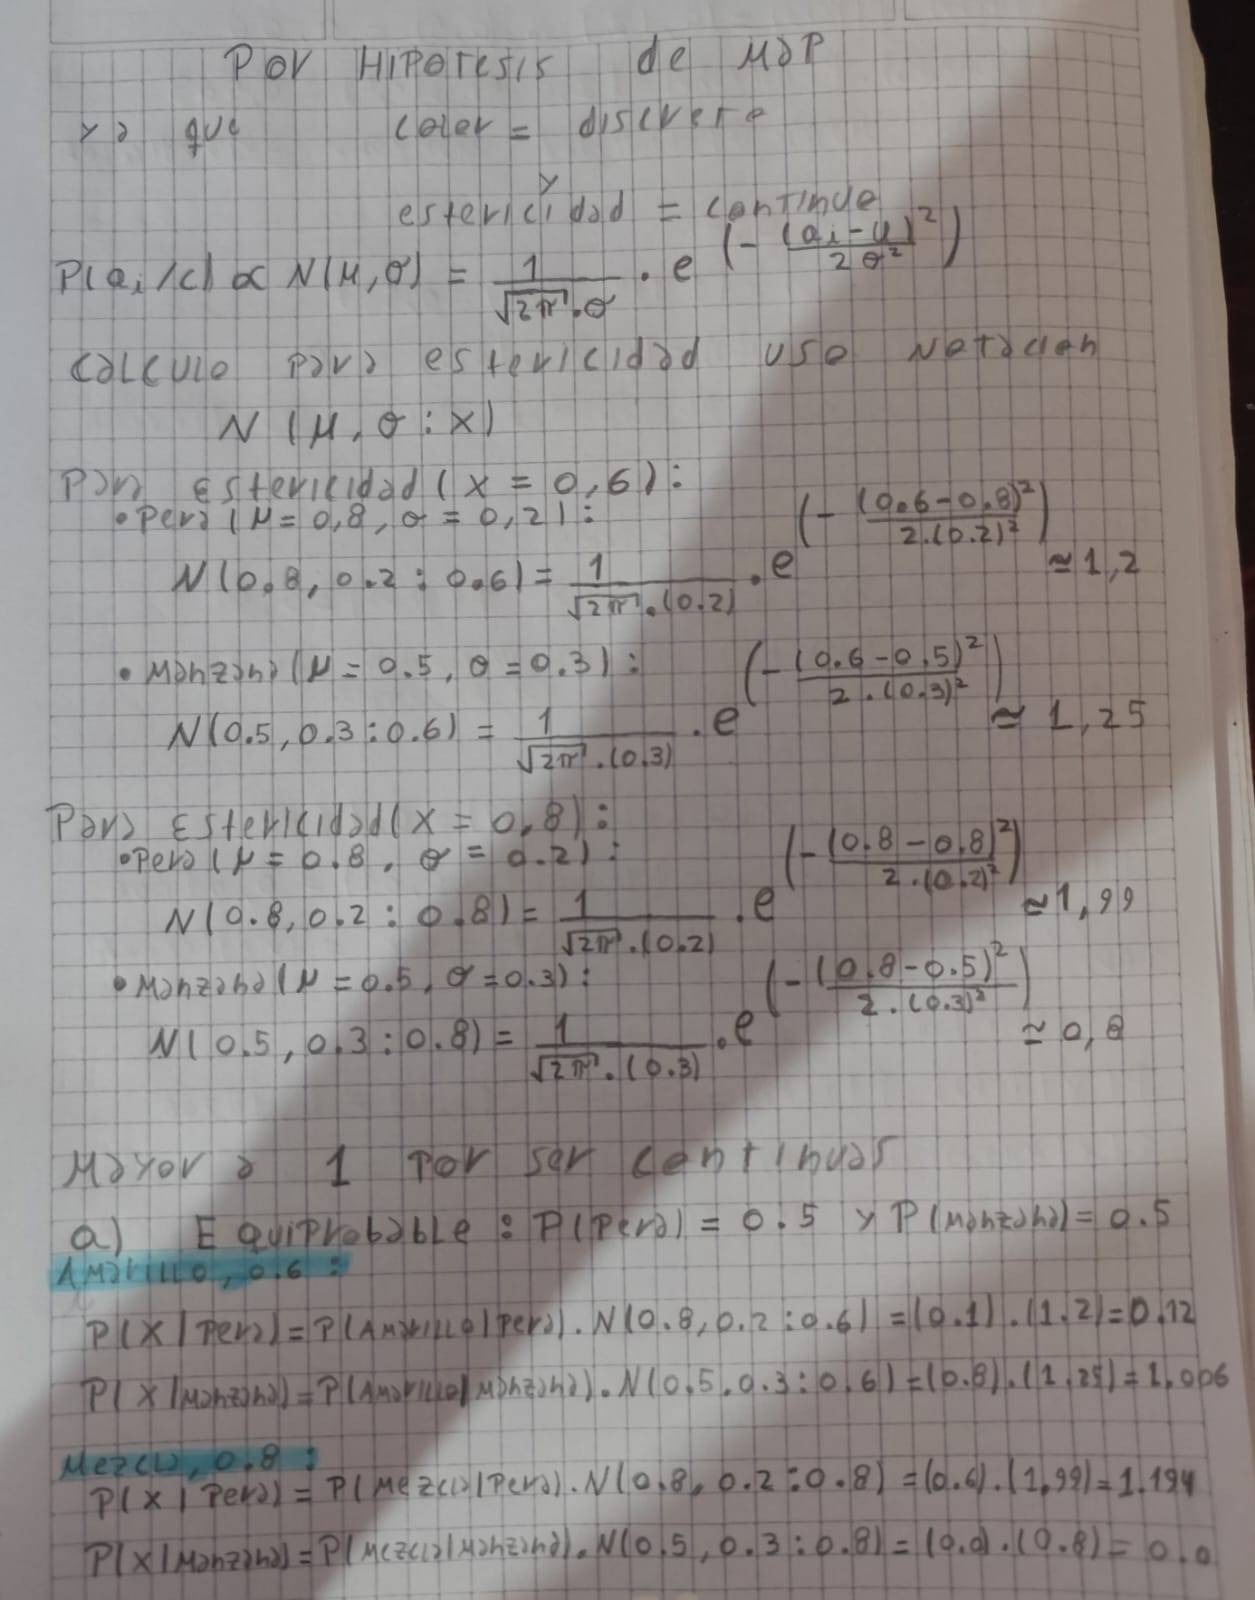
\includegraphics[width=0.9\textwidth]{4IncisoA.jpeg}
    \caption{Desarrollo manuscrito del Inciso A.}
\end{figure}

\begin{figure}[H]
    \centering
    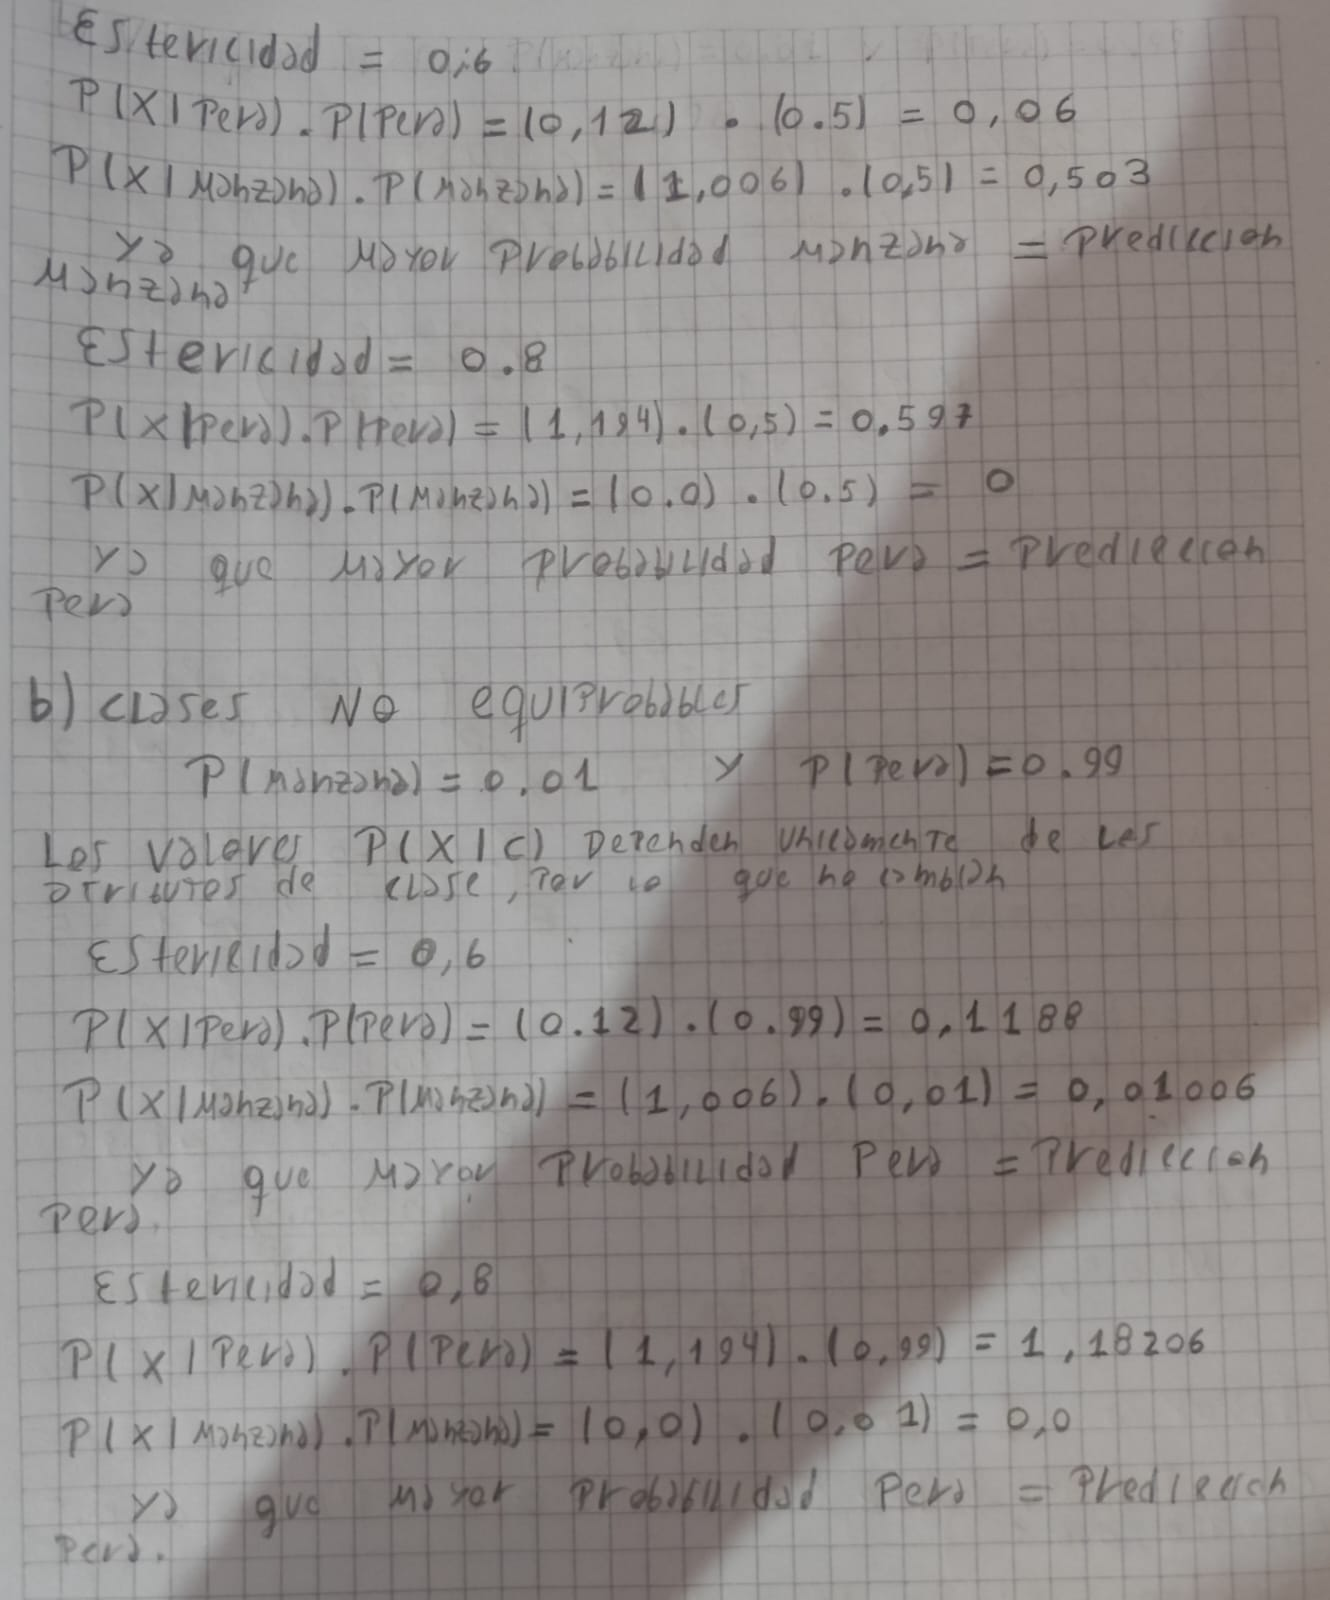
\includegraphics[width=0.9\textwidth]{4IncisoB.jpeg}
    \caption{Desarrollo manuscrito del Inciso B.}
\end{figure}

\begin{figure}[H]
    \centering
    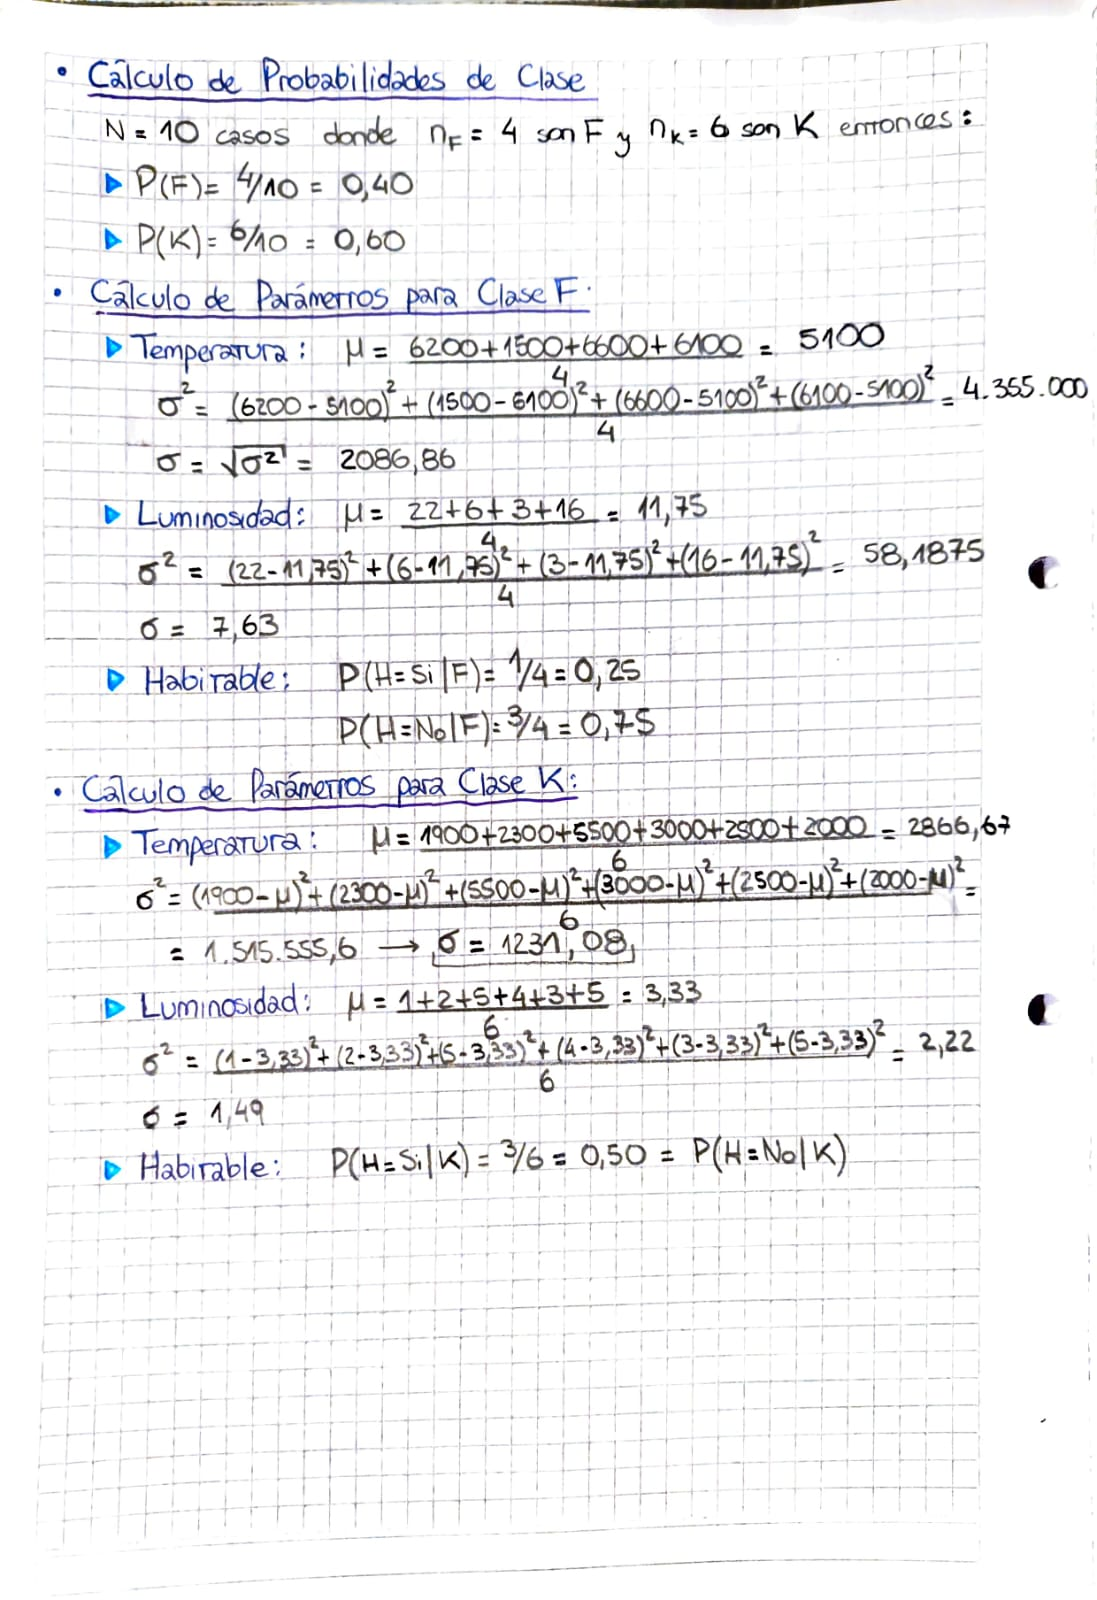
\includegraphics[width=0.9\textwidth]{5IncisoA.jpeg}
    \caption{Desarrollo manuscrito del Inciso A.}
\end{figure}

\begin{figure}[H]
    \centering
    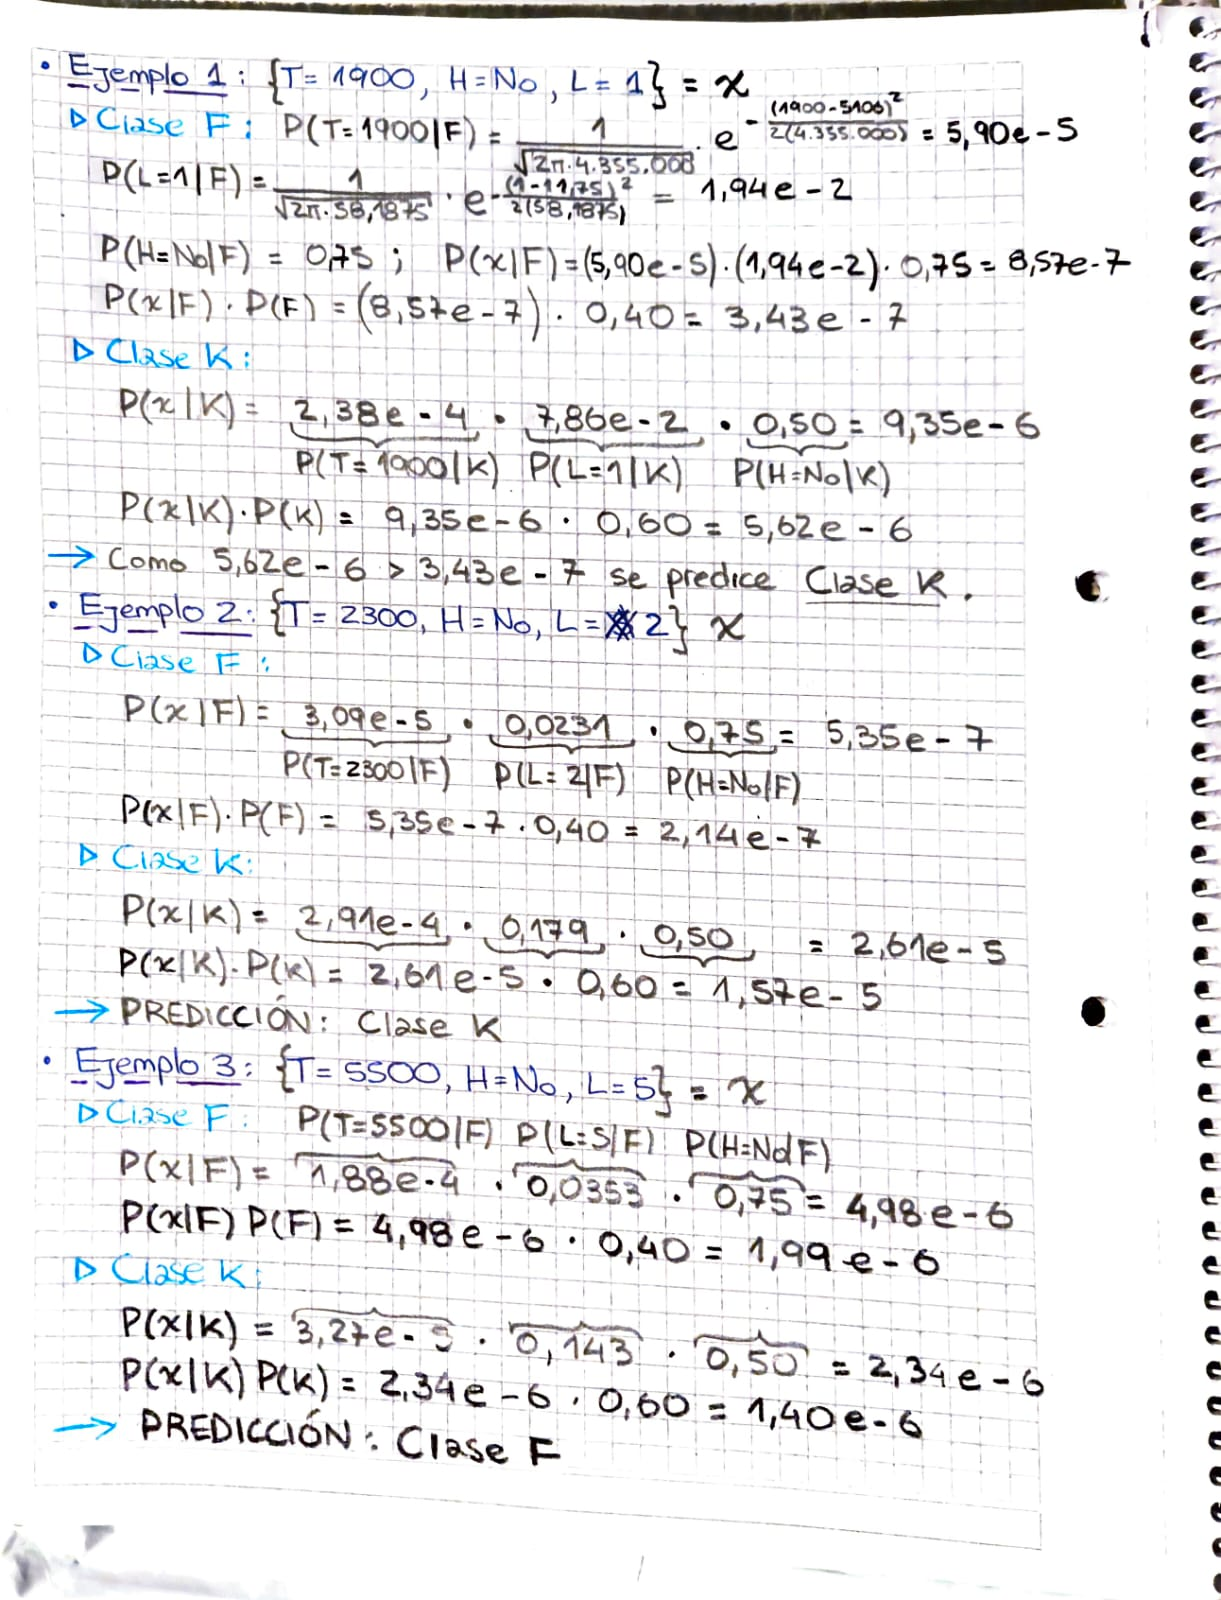
\includegraphics[width=0.9\textwidth]{5IncisoB.jpeg}
    \caption{Desarrollo manuscrito del Inciso B.}
\end{figure}

\end{document}